% CREATED BY DAVID FRISK, 2016
% MODIFIED BY JAKOB JARMAR, 2016
% A few changes by Birgit Grohe, 2017 and 2018
% Adjustments with the help of Gustav Örtenberg 2019

% IMPORT SETTINGS
\documentclass[12pt,a4paper,twoside,openright]{toptesi}
% CREATED BY DAVID FRISK, 2016

% BASIC SETTINGS
\usepackage{moreverb}								% List settings
\usepackage{textcomp}								% Fonts, symbols etc.
\usepackage{lmodern}								% Latin modern font
\usepackage{helvet}									% Enables font switching
\usepackage[T1]{fontenc}							% Output settings
\usepackage[english]{babel}							% Language settings
\usepackage[utf8]{inputenc}							% Input settings
\usepackage{amsmath}								% Mathematical expressions (American mathematical society)
\usepackage{amssymb}								% Mathematical symbols (American mathematical society)
\usepackage{graphicx}								% Figures
\usepackage{subfig}									% Enables subfigures
\numberwithin{equation}{chapter}					% Numbering order for equations
\numberwithin{figure}{chapter}						% Numbering order for figures
\numberwithin{table}{chapter}						% Numbering order for tables


\usepackage{chemfig}		% Chemical structures
\usepackage[top=3cm, bottom=3cm,
			inner=3cm, outer=3cm]{geometry}			% Page margin lengths			
\usepackage{eso-pic}								% Create cover page background
\newcommand{\backgroundpic}[3]{
	\put(#1,#2){
	\parbox[b][\paperheight]{\paperwidth}{
	\centering
	\includegraphics[width=\paperwidth,height=\paperheight,keepaspectratio]{#3}}}}
\usepackage{float} 									% Enables object position enforcement using [H]
\usepackage{parskip}								% Enables vertical spaces correctly 
\usepackage{datetime} %date formatting tools

%\usepackage{minted} 		% Enables source code listings


% OPTIONAL SETTINGS (DELETE OR COMMENT TO SUPRESS)

% Disable automatic indentation (equal to using \noindent)
\setlength{\parindent}{0cm}                         


% Caption settings (aligned left with bold name)
\usepackage[labelfont=bf, textfont=normal,
			justification=justified,
			singlelinecheck=false]{caption} 		

		  	
% Activate clickable links in table of contents  	
\usepackage{hyperref}								
\hypersetup{colorlinks, citecolor=black,
   		 	filecolor=black, linkcolor=black,
    		urlcolor=black}


% Define the number of section levels to be included in the t.o.c. and numbered	(3 is default)	
\setcounter{tocdepth}{5}							
\setcounter{secnumdepth}{5}	


% Chapter title settings
\usepackage{titlesec}		
\titleformat{\chapter}[display]
  {\Huge\bfseries\filcenter}
  {{\fontsize{50pt}{1em}\vspace{-4.2ex}\selectfont \textnormal{\thechapter}}}{1ex}{}[]


% Header and footer settings (Select TWOSIDE or ONESIDE layout below)
\usepackage{fancyhdr}								
\pagestyle{fancy}  
\renewcommand{\chaptermark}[1]{\markboth{\thechapter.\space#1}{}} 


% Select one-sided (1) or two-sided (2) page numbering
\def\layout{2}	% Choose 1 for one-sided or 2 for two-sided layout
% Conditional expression based on the layout choice
\ifnum\layout=2	% Two-sided
    \fancyhf{}			 						
	\fancyhead[LE,RO]{\nouppercase{ \leftmark}}
	\fancyfoot[LE,RO]{\thepage}
		\renewcommand{\footrulewidth}{0.4pt}
	\fancyfoot[C]{Chalmers University Of Technology}
	\fancyfoot[RE,LO]{\textit{Francesco Angione}}	
	\fancypagestyle{plain}{			% Redefine the plain page style
	\fancyhf{}
	\renewcommand{\headrulewidth}{0pt}
	\renewcommand{\footrulewidth}{0.4pt}
	\fancyfoot[LE,RO]{\thepage}
	\fancyfoot[C]{Chalmers University Of Technology}
	\fancyfoot[RE,LO]{\textit{Francesco Angione}}
	}	
	\fancypagestyle{plain_cover}{
	\fancyhf{}
	\renewcommand{\headrulewidth}{0pt}
		\renewcommand{\footrulewidth}{0pt}
	\fancyfoot[LE,RO]{\thepage}
	}
\else			% One-sided  	
  	\fancyhf{}					
	\fancyhead[C]{\nouppercase{ \leftmark}}
	\fancyfoot[C]{\thepage}
		\fancyfoot[C]{Chalmers University Of Technology}
	\fancyfoot[RE,LO]{\textit{Francesco Angione}}}	
\fi


% Enable To-do notes
\usepackage[textsize=tiny]{todonotes}   % Include the option "disable" to hide all notes
\setlength{\marginparwidth}{2.5cm} 


% Supress warning from Texmaker about headheight
\setlength{\headheight}{15pt}		

%  use bibtex references 
%, 
 \usepackage[backend=bibtex,  citestyle=numeric-comp,sorting=none,style=chem-angew ,articletitle=true]{biblatex}
 
 \usepackage{float}
 
 %for figure
 \usepackage{caption}


 
 \usepackage{epigraph}

\usepackage{tikz}
\usetikzlibrary{automata,positioning}

\usepackage{listings}

\usepackage{xcolor}


\lstdefinestyle{verilog-style}
{
    language=Verilog,
    basicstyle=\small\ttfamily,
    keywordstyle=\color{blue},
    identifierstyle=\color{black},
    commentstyle=\color{green},
    numbers=left,
    numberstyle=\tiny\color{black},
    numbersep=10pt,
    tabsize=8,
    moredelim=*[s][\colorIndex]{[}{]},
    literate=*{:}{:}1
}

\makeatletter
\newcommand*\@lbracket{[}
\newcommand*\@rbracket{]}
\newcommand*\@colon{:}
\newcommand*\colorIndex{%
    \edef\@temp{\the\lst@token}%
    \ifx\@temp\@lbracket \color{black}%
    \else\ifx\@temp\@rbracket \color{black}%
    \else\ifx\@temp\@colon \color{black}%
    \else \color{vorange}%
    \fi\fi\fi
}
\makeatother




\definecolor{veryLightGrey}{rgb}{0.9629411,0.9629411,0.9629411}
	
\lstset{language=C++,
        alsolanguage=[ANSI]C,
	keywordstyle=\color{vblue},
	keywordstyle=[2]\color{red},
	alsoletter={[2]\#},
	morekeywords={[2]\#include},
	basicstyle=\small\sffamily,
	commentstyle=\color{green}\small\sffamily,
	stringstyle=\sffamily,
	showstringspaces=false,
	breaklines=true,
	frame=none,
	numbers=left,                    % where to put the line-numbers; possible values are (none, left, right)
  numbersep=5pt,                   % how far the line-numbers are from the code
  numberstyle=\tiny\color{commentsColor}
  }


\setlength\epigraphwidth{10cm}
\setlength\epigraphrule{0pt}


%% for centering in the tables
\usepackage{array}
\newcolumntype{P}[1]{>{\centering\arraybackslash}p{#1}}






\usepackage{adjustbox} % to resize boxes by keeping the same aspect ratio
%\usepackage{algorithm} % algorithm environment
%\usepackage{geometry}
\usepackage{mfirstuc} % to have capitalization capabilities
\usepackage[final]{microtype}      % microtypography, final lets latex use it also in bibliography
%\usepackage{siunitx} % support for SI units of measurement and number typesetting


% change this configuration with your info
% if you need fewer or more supervisors you have to change \relatore command by adding or removing lines in the table in toptesi_config
\newcommand{\thesistitle}{A FPGA-based tensor accelerator for Machine Learning}
\newcommand{\thesisuniversitylogo}{logoPoliTo_symbol_only} % choose your logo
\newcommand{\thesiscandidatename}{Francesco }
\newcommand{\thesiscandidatesurname}{Angione }
\newcommand{\thesissupervisoronetitle}{prof.}
\newcommand{\thesissupervisoronename}{Paolo}
\newcommand{\thesissupervisoronesurname}{Bernardi}
\newcommand{\thesissupervisortwotitle}{prof.}
\newcommand{\thesissupervisortwoname}{Pedro P.M.}
\newcommand{\thesissupervisortwosurname}{Trancoso}
\newcommand{\thesisdate}{A.Y. 2019/2020}
\newcommand{\thesiscourse}{Computer Engineering}
\newcommand{\thesisuniversity}{Politecnico di Torino}
\newcommand{\thesislevel}{Master} % master or bachelor
\newcommand{\thesiscandidatetext}{Candidate}
\newcommand{\thesissupervisortext}{Supervisors}


\bibliography{./include/backmatter/references.bib}


\begin{document} 
% COVER PAGE, TITLE PAGE AND IMPRINT PAGE

%% CREATED BY DAVID FRISK, 2016
% MODIFIED BY JAKOB JARMAR, 2016
% A few changes by Birgit Grohe, 2017 and \the\year
% Adjustments with the help of Gustav Örtenberg 2019

% COVER PAGE
\begin{titlepage}
\newgeometry{top=3cm, bottom=3cm,
			left=2.25 cm, right=2.25cm}	% Temporarily change margins		
			
% Cover page background 
\AddToShipoutPicture*{\backgroundpic{-4}{56.7}{figure/auxiliary/frontpage_gu_eng_vec_m2.pdf}}
\addtolength{\voffset}{2cm}

% Cover picture (replace with your own or delete)		
\begin{figure}
\centering
\vspace{1cm}	% Adjust vertical spacing here
\includegraphics[scale=1]{figure/cover.jpg}
\end{figure}

% Cover text
\mbox{}
\vfill
\renewcommand{\familydefault}{\sfdefault} \normalfont % Set cover page font

\textbf{\Huge  \multiLineTitle{0.2cm}}\\[0.5cm]

%{\Large aaa \oneLineSubtitle}\\[0.5cm]

%{\Large A Subtitle that can be Very Much Longer if Necessary}\\[0.5cm]

Erasmus Master thesis in Computer science engineering \setlength{\parskip}{1cm}

{\Large Francesco Angione} \setlength{\parskip}{2.9cm}

Department of Computer Science and Engineering \\
\textsc{Chalmers University of Technology} \\
\textsc{University of Gothenburg} \\
Gothenburg, Sweden \the\year

\renewcommand{\familydefault}{\rmdefault} \normalfont % Reset standard font
\end{titlepage}


% BACK OF COVER PAGE (BLANK PAGE)
\newpage
\restoregeometry
\thispagestyle{empty}
\mbox{}


% TITLE PAGE
\newpage
\thispagestyle{empty}
\begin{center}
	\textsc{\large Master's thesis \the\year}\\[4cm]		% Report number is currently not in use
	\textbf{\Large \multiLineTitle{0.2cm}} \\[1cm]
%	{\large  \oneLineSubtitle }\\[1cm]
	{\large Francesco Angione}
	
	\vfill	
	% Logotype on titlepage	
	\begin{figure}[H]
	\centering
	% Remove the following line to remove the titlepage logotype
	%\includegraphics[width=0.25\pdfpagewidth]{figure/auxiliary/ChGULogoHog.pdf}
	\end{figure}	\vspace{5mm}	
	
	Department of Computer Science and Engineering\\
	%\emph{Division of Division name}\\
	%Name of research group (if applicable)\\
	\textsc{Chalmers University of Technology} \\
	\textsc{University of Gothenburg} \\
	Gothenburg, Sweden \the\year \\
\end{center}


% IMPRINT PAGE (BACK OF TITLE PAGE)
\newpage
\thispagestyle{empty}
\vspace*{4.5cm}
%\oneLineTitle\\
%\oneLineSubtitle\\
%Francesco Angione\setlength{\parskip}{1cm}

%\copyright ~ Francesco Angione, \the\year. \setlength{\parskip}{1cm}

Supervisor: Pedro Petersen Moura Trancoso, Department of Computer Science and Engineering, Chalmers University of Technology \\
Home Supervisor: Paolo Bernardi,  Department of Control and Computer Engineering, Polytechnic of Turin \\
Examiner: Per Larsson-Edefors ,Department of Computer Science and Engineering, Chalmers University of Technology  \setlength{\parskip}{1cm}

Master's Thesis \the\year\\	% Report number currently not in use 
Department of Computer Science and Engineering\\
%Division of Division name\\
%Name of research group (if applicable)\\
Chalmers University of Technology\\
SE-412 96 Gothenburg\\
Telephone +46 31 772 1000 \setlength{\parskip}{0.5cm}

\vfill
% Caption for cover page figure if used, possibly with reference to further information in the report
Cover: A robot involved into the self learning process, reading.


%Typeset in \LaTeX \\
%Printed by [Name of printing company]\\
%Gothenburg, Sweden \the\year


% fontsize is {size}{spacing}\family
\ateneo{\thesisuniversity} % university name
\logosede[5cm]{\thesisuniversitylogo} % logo, square brackets contain the height

\titolo{\thesistitle} % title
%\sottotitolo{Metodo dei satelliti medicei} % subtitle

% place/remove a slash \\ to put the name on the following line or after Master Degree Course
\corsodilaurea{\thesiscourse} % course name


%~251197 % id number is not needed

\candidato{\thesiscandidatename~\textsc{\thesiscandidatesurname}} % candidate

% using tabular we can have more than 1 supervisor under the same column
\relatore{\tabular{@{}l}%
    \xmakefirstuc{\thesissupervisoronetitle}~\thesissupervisoronename~\textsc{\thesissupervisoronesurname}\\[0.4ex]
    \xmakefirstuc{\thesissupervisortwotitle}~\thesissupervisortwoname~\textsc{\thesissupervisortwosurname}\\[0.4ex]
   % \xmakefirstuc{\thesissupervisorthreetitle}~\thesissupervisorthreename~\textsc{\thesissupervisorthreesurname}
    \endtabular}


% in this way we have Academic Year without stile=classica, so without lines
%\sedutadilaurea{\textsc{Academic~Year} 2019-2020}% per la laurea magistrale
% for PoliTo there is only month year
\sedutadilaurea{\thesisdate}% per la laurea magistrale
% PhD
%\esamedidottorato{Novembre 1610}
%\ciclodidottorato{XV}

% offset for binding, the smaller the better
%\setbindingcorrection{3mm}


\english% or \italian (default)

\iflanguage{english}{%
	%\retrofrontespizio{This work is subject to the Creative Commons Licence}

	\CorsoDiLaureaIn{\thesislevel's Degree Course in\space}

	\TesiDiLaurea{\thesislevel's Degree Thesis}

	\InName{in}
	\CandidateName{\xmakefirstuc{\thesiscandidatetext}}% or Candidates
	\AdvisorName{\xmakefirstuc{\thesissupervisortext}}% or Supervisor
	%\TutorName{Tutor}
	%\NomeTutoreAziendale{Internship Tutor}

	%\NomePrimoTomo{First volume}
	%\NomeSecondoTomo{Second Volume}
	%\NomeTerzoTomo{Third Volume}
	%\NomeQuartoTomo{Fourth Volume}
}{}
\pagenumbering{roman}			% Roman numbering (starting with i (one)) until first main chapter
%polito front page
\newgeometry{top=4cm,left=3cm,right=3cm,bottom=4cm,heightrounded}
\begin{titlepage}
\centering
%
{\fontsize {22}{30}\scshape \textbf{\MakeUppercase{\thesisuniversity}} \par}
%
\vspace{\stretch{2}} % changing this number and the others changes the proportion
%
{\fontsize {16}{20}\rmfamily \textbf{\thesislevel's Degree in \thesiscourse} \par}
%
\vspace{\stretch{3}}
%
\includegraphics[width=50mm]{\thesisuniversitylogo}\\
%
\vspace{\stretch{4}}
%
{\fontsize {16}{20}\rmfamily \textbf{\thesislevel's Degree Thesis} \par}
%
\vspace{\stretch{3}}
%
{\fontsize {21}{28}\scshape \textbf{\thesistitle} \par}
%
\vspace{\stretch{10}}
%
\makebox[\textwidth]{\null\hfill\def\arraystretch{2}% % to change the spacing change this number
\begin{minipage}[t]{.375\textwidth}\raggedright
    \begin{adjustbox}{width={\textwidth},totalheight={\textheight},keepaspectratio} % with adjustbox it adapts to the lengths of the names, remove it if you want the same font dimension
    \begin{tabular}[t]{@{}l@{}}
        \fontsize {14}{20}\mdseries \textbf{\thesissupervisortext} \\
        \fontsize {14}{20}\bfseries \xmakefirstuc{\thesissupervisoronetitle}~\thesissupervisoronename~\MakeUppercase{\thesissupervisoronesurname}\\
       \fontsize {14}{20}\bfseries \xmakefirstuc{\thesissupervisortwotitle}~\thesissupervisortwoname~\MakeUppercase{\thesissupervisortwosurname}\\
       % \namesfont \xmakefirstuc{\thesissupervisorthreetitle}~\thesissupervisorthreename~\MakeUppercase{\thesissupervisorthreesurname}
    \end{tabular}
    \end{adjustbox}
\end{minipage}
%
\hfill
%
\begin{minipage}[t]{.375\textwidth}\raggedleft
\begin{adjustbox}{width={\textwidth},totalheight={\textheight},keepaspectratio} % with adjustbox it adapts to the lengths of the names, remove it if you want the same font dimension
\begin{tabular}[t]{@{}l@{}}
    \fontsize {14}{20}\mdseries \textbf{\thesiscandidatetext} \\
    \fontsize {14}{20}\bfseries \thesiscandidatename~\MakeUppercase{\thesiscandidatesurname}
\end{tabular}
\end{adjustbox}
\end{minipage}\hfill\null}\\
%
\vspace{\stretch{5}}
%
{\fontsize {15}{18}\rmfamily \textbf{\thesisdate} \par}
%
\end{titlepage}

\restoregeometry % custom frontpage
\paginavuota


% ABSTRACT
\newpage
% CREATED BY DAVID FRISK, 2016
%\oneLineTitle\\
%\oneLineSubtitle\\
%NAME FAMILYNAME\\
%Department of Computer Science and Engineering\\
%Chalmers University of Technology and University of Gothenburg\setlength{\parskip}{0.5cm}

\thispagestyle{plain_cover}			% Supress header 
\setlength{\parskip}{0pt plus 1.0pt}
\section*{Abstract}

\todo[inline]{Abstract text about your project in  Computer Science and Engineering.}

\todo[inline]{add cover image}

% KEYWORDS (MAXIMUM 10 WORDS)
%\vfill
%Keywords: Computer, science, computer science, engineering, project, thesis.

\newpage				% Create empty back of side
\thispagestyle{empty}
\mbox{}

% ACKNOWLEDGEMENTS
\newpage
% CREATED BY DAVID FRISK, 2016
\thispagestyle{plain_cover}			% Supress header
\section*{Acknowledgements}
 
 It is always hard to write this part of a work. I would say it is the hardest part, more than the technical one.\\ 
However, let me try to address it anyway. I am apologizing in advance if i will forgot something.\\\\
 
This work has been developed during a 

sum of all experience form a technical poitn of view and life

This work has also taught that we are just human, but we can do whatever we can image, especially in Computer Science.

cause we are just human, but we can do whatever we can image.

I would like to thank to both my supervisors Prof. Paolo Bernardi and Prof. Pedro Petersen Moura Trancoso for believing in me without any guarantees on the final work, and their support through this journey.\\

\textit{
To the day in which I learnt how to read, an important pillar of my life.\\
To the people who have contribuited, in badness and goodness, to make the person who i am today.\\
To my past and future failures, where i have built and i will build myself.\\
To my feelings, which remembers us how much we are fragile but at the same time they remind us we are human being and we gather our strength.\\
Sapere aude.\\}

\vspace{1.5cm}
\hfill
Francesco Angione, Gothenburg, \monthname \space \the\year

\newpage				% Create empty back of side
\thispagestyle{empty}
\mbox{}


% TABLE OF CONTENTS
\newpage
\tableofcontents

% OTHER FRONTMATTER
% List of figures (add to table of contents)
\cleardoublepage
\addcontentsline{toc}{chapter}{\listfigurename} 
\listoffigures
% List of tables (add to table of contents)
\cleardoublepage
\addcontentsline{toc}{chapter}{\listtablename}  
\listoftables


% START OF MAIN DOCUMENT
\cleardoublepage
\setcounter{page}{1}
\pagenumbering{arabic}			% Arabic numbering starting from 1 (one)
\setlength{\parskip}{0pt plus 1pt}

% INTRODUCTION
% CREATED BY DAVID FRISK, 2016
\chapter{Introduction}
Machine learning is one of the hot technologies today as it is being used to solve complex problems that would otherwise be very hard or costly to solve with traditional methods. Speech and image recognition, as well as many other complex decision-making problems such as self-driving vehicles are successfully solved with machine learning and deep-learning. 
The success of machine learning is being driven by the current available hardware which can provide the required demands in terms of storage and compute capacity. But obviously as problems scale so do the demands and thus special hardware is being developed to address these needs. \\\\
The use of commodity hardware is not the most effective and efficient way to address this problem, so research is looking at solution that can satisfy the required demands but at lower cost and energy consumption in order to support machine learning also on mobile devices.
The constant developments in the machine learning methods require the design of more flexible hardware accelerators \cite{paper:1} \cite{paper:2}.\\
As it is very well-known, hardware accelerators are capable, if designed correctly, of delivering a lot of improvements in terms of the latency but also in terms of energy efficiency\cite{paper:29}. Thus, in order to obtain the best solution in every metric a hardware-software co-design is needed, requiring to the designer a basic knowledge of machine learning algorithms.\\\\

In the last years, the number of published papers regarding Machine Learning has growth exponentially, leading to significant efforts also from the companies which started to develop, deploy and sell their own hardware platforms, such as Tensor Processing Unit \cite{paper:40} from Google, NVDLA\cite{WEBSITE:6} from Nvidia and Gaudi \cite{paper:39} and Goya\cite{paper:38}, respectively for training and interference, from Habana (acquired by Intel).\\\\
Machine Learning includes two processes, the training and the inference. Mainly, the work is focused on the inference process, exploring different optimizations in terms of hardware.\\\\The goal is to develop an hardware accelerator for the inference process of Machine Learning applications, which is also configurable in terms of arithmetic precision for accomodating different precision requests from different models. Most of the computations in the inference process are composed of multiply and accumulate of data, where some of them are often reused, the accelerator will speed-up those aspects, exploiting a non Von-Neumann architecture. It is designed from scratch, therefore the work is carried out on FPGA in order to have the possibility of exploring different solutions and measuring different design metrics of the prototype. Integrating the hardware with an high level ML-FrameWork will also allow to meausure the overall latency of the Neural Network model for real time application and compare performances with different accelerator size for finding the best trade-off for a mobile device.\\\\
One of the main ideas of the work is that during the inference process, a model does not need high precision computations \cite{paper:8} \cite{paper:15}for achieving high accuracy into its outputs. Thus, the use of different arithmetic data type can drastically reduce the computations without reducing the final accuracy of the DNN \cite{paper:7} \cite{paper:8}. From a hardware perspective,  the use of different arithmetic precision\cite{paper:14}, such as the use of integer operations instead of floating point operations, can lead to benefits in terms of area, energy consumption and latency. Following the benefits previosly mentioned, the final system may be deployed on energy-area constrained devices. Moreover, the possibility of decide the current arithmetic precision of the accelerator allows the user, or the high level application, to use different neural network models leading to the use of different  applications and/or domains of the same hardware, or even at the same time from the user perspective, actually the two models could be multiplexed in time on the accelerator.\newline
According to that, accuracy of operations, reliability, performance and energy efficiency are evaluated, moving through different designs with different precision and compared to the implementation of the same DNN inside a GPU, as well as custom hardware platform.


Please organize better your thoughts. You can not have a goal and then a "main idea"... specify clearly what do you want. TO build an accelerator. Then that it is energy efficient. What do you do for that? You use FPGA as a technology for easy reconfiguration and flexibility and also you explore using limited precision for more energy efficiency!
Also please state clearly a "research question" that you plan to answer with your work!


% THEORY
% CREATED BY DAVID FRISK, 2016
\chapter{Background}
\textit{In this chapter a general glance on Artificial Intelligence, and its sub-categories , is given.}\\\\


\epigraph{ \textit{Can a machine think?}}{--- \textup{Alan Turing}, Computing Machinery and Intelligence}

\section{Overview}

description and reasoning of AI in general 

figure of division 

\subsection{Machine Learning}
 description 
 
 \subsubsection{Brain Inspired}
 
\subsubsection{Neural Networks}

\subsubsection{Deep Learning}

 math model 
 
 
\section{Applications}



% State of art
\chapter{State-of-the-Art}
\section{Overview}
The role of Machine Learning has continuously growth in the past few years and a lot of efforts has been done for developing good software APIs in order to address different needs and domains. \newline In principle, all the machine learning algorithms can be run on the CPU, which already runs the OS and other Application Software, this leads to a lot of overheads, especially in terms memory accesses which are expensive in terms of energy and latency. \\\\
Analyzing machine learning algorithms it comes evident that they massively do the same operations and access to data with some kind of patterns. Thus, with the outcome of the new paradigm for the GPU, the General Purpose GPU programming it comes in handy that implementing those algorithms on a GPU, which matches the Machine Learning algorithms requirements regarding the massive operations and the reuse of data, has given a lot of advantages in terms of latency and energy efficiency. However, the capability of GPU of running machine learning algorithms has been pushed almost at the maximum with the increase of computation demands in modern neural networks, therefore other solutions have been explored, such as the development of specific hardware platform.

\section{GPU}
The Moore's law is reaching the end from the point of view of CPUs. However, it seems that the GPUs can still carry on the Moore's law \cite{5496638}.\newline
For this reason, a lot of improvements especially from the companies have been made for developing more and more GPUs with a lower performance per watts.\\
As already mentioned, with the income of general purpose GPU programming paradigm, more and more machine learning algorithms have been designed for being run on the GPU, gathering the best fruits given by that type of architecture.\\\\
As consequences, companies such as Nvidia have started to develop GPU for boosting machine learning applications performance.
\subsection{Nvidia Ampere A100 Tensor Core GPU}
The Nvidia Ampere A100 Tensor Core GPU has been announcer recently and it is one of the most performant GPU. The newly added Tensor Core Unit allows massive increases in throughput and efficiency.\\It is able to deliver up to 624 TFPLOPS\footnote{floating-point operations per second} for training and inference machine learning applications.\\\\

The GPU is composed of multiple GPU processing clusters (GPCs), texture processing clusters (TPCs) and streaming multiprocessors (SMs).
The core of the GPU is the Streaming Multiprocessor, which is built up from the SM of Volta GPU and Turing one.
\begin{figure}[!htbp]
\centering
\captionsetup{justification=centering}
\includegraphics[scale=0.6]{./figure/volta_sm_arch.PNG}
\caption{Streaming Multiprocessor Architecture \cite{paper:41}}
\label{fig:voltasmarch}
\end{figure}

Composed of integer, FP32, FP64 units and the Tensor Core Units designed specifically for deep learning. It introduces also new data types in the tensor core for the computation, binary, integer 8 and 4 bits, floating-point 64, 32, 16 and bfp16 (the throughput of the tensor core computation for fp16 and bfp16 is the same). The Ampere SM can achieve such efficient workload on mixed computation and addressing calculations thanks to an independent parallel integer and floating-point data paths. \\\\

Matrix-Matrix multiplication operations are at the core of neural network training and inference, and are used to multiply large matrices of input data and weights in the connected layers of the network. The idea is represented into the Figure \ref{fig:tensorcorevolta} and compared to previous architectures.

\begin{figure}[!htbp]
\centering
\captionsetup{justification=centering}
\includegraphics[scale=0.6]{./figure/tensor_core.PNG}
\caption{Matrix Multiplication in Tensor Core\cite{paper:41}}
\label{fig:tensorcorevolta}
\end{figure}

The Ampere A100 GPU contains 108 Streaming multiprocessor, and 432 third generation Tensor Core.
According to Figure \ref{fig:mixprec} the Tensor Core Units are able to compute multiplications on FP16 and accumulate on FP32, leading to a further reduction of latency and energy consumption.
\begin{figure}[!htbp]
\centering
\captionsetup{justification=centering}
\includegraphics[scale=0.8]{./figure/mix_prec.PNG}
\caption{Mixed Precision Schema of a FMA unit in Tensor Core Unit\cite{paper:41}}
\label{fig:mixprec}
\end{figure}

A novel approach for doubling the throughput of deep neural networks has been introduced in this architecture. At the end of training process, only a subset of the total weights are necessary to execute a neural network correctly. As consequence not all the weights are needed, and they can be removed.\\
Based on training feedback, weights can be adapted at runtime during the training and this does not have any impact on the final accuracy. Thus, thanks to the sparsity of weight tensors., inference process can be accelerated. In addition, also the training process can be accelerated exploiting the sparsity idea but it has to be introduced at the beginning of the process for achieving some benefits.

\begin{figure}[!htbp]
\centering
\captionsetup{justification=centering}
\includegraphics[scale=0.4]{./figure/sparsity.png}
\caption{Sparsity Optmization of a weight tensor\cite{paper:41}}
\label{fig:spa}
\end{figure}
The apporach in Fig. \ref{fig:spa} doubles the throughput by skipping the zeros, it also leads to a reduction of memory footprint and an increase into the memory bandwidth.\\

Following the idea, NVIDIA has introduced a new set of instruction for inference: sparse Matrix Multiply-Accumulate (MMA). Those instructions are able to skip the matrix entries which contain zero values leading to an increase of the Tensor core throughput. An example can be seen in Fig. \ref{fig:mma}, where the light blue matrix has a sparsity of 50\%. It is also important to mention that the non-zero entries of the light blue matrix will be matched with the correct entries of the red one.
\begin{figure}[!htbp]
\centering
\captionsetup{justification=centering}
\includegraphics[scale=0.35]{./figure/mma.png}
\caption{Matrix Multiply Accumulate\cite{paper:41}}
\label{fig:mma}
\end{figure}

\newpage
The deep learning frameworks and the CUDA Toolkit include libraries that have been custom-tuned to provide high multi-GPU performance for each one of the following deep learning frameworks in the Figure \ref{fig:swtesla}.

\begin{figure}[!htbp]
\centering
\captionsetup{justification=centering}
\includegraphics[scale=0.6]{./figure/sw_stack_tesla.PNG}
\caption{Software stack\cite{paper:41}}
\label{fig:swtesla}
\end{figure}

Combining powerful hardware with software tailored to deep learning, it provides to developers and researchers solutions for high-performance GPU-accelerated deep learning application development, testing, and network training.
\newpage
\section{Domain Specific Hardware Platform}
Instead of developing GPUs also suitable for Machine Learning applications, the companies have designed and deployed special purpose hardware accelerators.
\subsection{NVDLA}
The Nvidia Deep Learning Accelerator is a free open source hardware platform from Nvidia, highly customizable and modular, which allows to design and deploy deep learning inference hardware.

The architecture comes in two configurations:

\begin{figure}[!htbp]
\centering
\captionsetup{justification=centering}
\includegraphics[scale=0.4]{./figure/nvdla_system.PNG}
\caption{Comparsion of two possible NVDLA system\cite{WEBSITE:8}}
\label{fig:nvdlasystem}
\end{figure}
As already mentioned, the aim of the work is to develop a hardware accelerator for machine learning suitable for mobile devices, therefore from now on the NVDLA small system will be considered and analyzed.\\
The internal architecture of the NVDLA small system is:
\begin{figure}[!htbp]
\centering
\captionsetup{justification=centering}
\includegraphics[scale=0.5]{./figure/nvdla_internal.PNG}
\centering\caption{Internal architecture of NVDLA small system, Secondary DBB not considered\cite{WEBSITE:8}}
\label{fig:nvdlaarch}
\end{figure}

According to Figure \ref{fig:nvdlasystem}, for the Small configuration of the accelerator, the processor will be in charge of programming and scheduling the operations on the NVDLA and as consequences handles the start/end of operations and possible interrupts, all of them through the CSB (Configuration Space Bus) interface which is AXI Lite compliant\cite{paper:30}. \newline
The data movement to/from memory are handled by the Internal memory controller though the DBB (Data BackBone) interface, which is AXI \cite{paper:30} compliant.\\

The internal architecture of NVDLA is composed by various engines, each one of them is able to perform specific Machine Learning models:
\begin{itemize}
\item Convolution Core: it comes in pair with the Convolution Buffer, its private memory for the data (inputs and weights). It is used to accelerate the convolution algorithms.
\item Activation engine (Single Data point Operations): it performs post processing operations at the single data element level such as bias addition, Non-linear function, PReLU (Parametric Rectified Linear Unit) and format conversion when the software requires different precision for different hardware layers.
\item Pooling engine (Planar Data Operations): it is designed to accomplish pooling layers, i.e. it executes operation along the width and height plane.
\item Local response normalization engine(Cross Channel Data operations): it is designed to address local response normalization layers.
\item Reshape(Data memory and reshape operations): it transforms data mapping format without any data calculation.
\item Bridge DMA: it is in charge of copying data from the Main Memory to the SRAM of the accelerator, only available into the large configuration of the system.
\end{itemize}

Another possible configuration which is worth to mention is the possibility to let the engines work separately on independent task or in a fused fashion where all of them are pipelined, working as a single entity.\\

According to developers the configurability of the cores ranges from arithmetic precision to the theoretical throughput that a single unit can achieve (increasing the number of internal Processing Elements). Moreover, since the engine units are independent of each other, according to the application and the model used they can be safely removed from the design.
\newpage
\subsubsection{ NVDLA Software }
It is also worth to mention that the accelerator comes already with a basic software stack:
\begin{figure}[H]
\centering
\captionsetup{justification=centering}
\includegraphics[scale=0.8]{./figure/nvdla_software.PNG}
\caption{NVDLA Software stack\cite{WEBSITE:7}}
\label{fig:nvdlasw}
\end{figure}

Where the Compilation tools are in charge of converting existing pretrained model into a set of hardware layers (for the desired precision) and programming sequences suitable for the NVDLA, the output of this process is a Nvidia Loadable file suitable for the runtime environment.\\
Regarding the runtime environment, it has been designed for a system in which is present an OS. It is composed in two parts: the User Mode Driver (UMD) and the Kernel Mode Driver (KMD).\newline The User Mode Driver loads the loadable file in memory and submits the operation to the KMD, it is also in charge of data movement from/to the accelerator. \newline The KMD is in charge of submit operations to the accelerator through low level functions, schedules the operations and handles the interrupts.\\
Both the KMD and the UMD are wrapped into portability layers which are, respectively, hardware dependent and OS dependent. In principle, for migrating the software to another OS or hw plaftorm it is enough to modify only the portability layers.
\newpage
\subsection{Google TPU}
Google developed its own application-specific integragrated circuit for neural networks, which is tightly integrated with TensorFlow Software.
It includes:
\begin{itemize}
\item Matrix Multiplier Unit (MXU): 65,536 8-bit multiply-and-add units for matrix operations
\item Unified Buffer (UB): 24 MB of SRAM that work as registers
\item Activation Unit (AU): Hardwired activation functions
\end{itemize}

In Figure \ref{fig:tpuarch} a general view of TPU architecture is presented.
\begin{figure}[H]
\centering
\captionsetup{justification=centering}
\includegraphics[scale=0.8]{./figure/tpu_arch.PNG}
\caption{Google TPU architecture\cite{paper:40}}
\label{fig:tpuarch}
\end{figure}

Rather than be tightly integrated with a CPU, the TPU is designed to be a coprocessor in which the instruction are sent by the host server rather than fetched.\\\\
The matrix multiplication unit reuses both inputs many times as part of producing the output avoiding the overhead of continuously read data from memory. Only spatial adjacent ALU are connected together, which makes wires shorter and energy-efficient. The ALUs only perform computations in fixed pattern.
\newpage
As far as concern the software stack, the TPU can be programmed for a wide variety of neural network models. To program it, API calls from TensorFlow graph are converted into TPU instructions.
\begin{figure}[H]
\centering
\captionsetup{justification=centering}
\includegraphics[scale=0.4]{./figure/tpu_sw_stack.PNG}
\caption{Google TPU Software Stack\cite{WEBSITE:9}}
\label{fig:gtpuswstack}
\end{figure}

\subsection{Habana Goya HL-1000}

Habana’s Goya is a processor dedicated to inference workloads. It is designed to deliver superior performance, power efficiency and cost savings for data centers and other emerging applications.\\
It allows the adoption of different deep learning models and is not limited to specific domains. Moreover, the performance requirements and accuracy can be user-defined.\\

In the Figure \ref{fig:goyaarch} a high level view of the Goya architecture can be appreciated.
\begin{figure}[H]
\centering
\captionsetup{justification=centering}
\includegraphics[scale=0.7]{./figure/goya_arch.PNG}
\caption{High level view of Goya architecture\cite{paper:38}}
\label{fig:goyaarch}
\end{figure}

It is based on scalable, fully programmable Tensor Processing Cores, specifically designed for deep learning workloads. \\
It also provides other flexible features such as GEMM operation acceleration, special functions dedicated hardware, tensor addressing, latency hiding capabilities and different data types support in TPC (FP32, INT32, INT16, INT8, UINT32, UINT16, UINT8).\\

Regarding the software stack, it can be interfaced with all deep learning frameworks. However, a model has to be first converted into an internal representation, as it can be seen in Figure \ref{fig:goyaswstack}.
\begin{figure}[H]
\centering
\captionsetup{justification=centering}
\includegraphics[scale=0.5]{./figure/goya_sw_stack.PNG}
\caption{Habana Goya Software Stack\cite{paper:38}}
\label{fig:goyaswstack}
\end{figure}
It also supports quantization of models trained in floating-point format with near-zero accuracy loss.

% METHODS

% CREATED BY DAVID FRISK, 2016
\chapter{System Development}
\textit{In the following chapter a Top Down approach of the System development is described, with particular emphasis on the hardware development part.}
\section{Overview}
\todo{it should start with a justification and overview of the proposed accelerator}
The entire work is implemented on a PYNQ Z2 board from TUL, based on a Zynq-7000 SoC \cite{paper:31}.

\begin{figure}[!htbp]
\centering
\captionsetup{justification=centering}
\includegraphics[scale=0.35]{./figure/zynq.PNG}
\caption{Zynq 7000 SoC\cite{paper:42}}
\label{fig:zynq}
\end{figure}

The latter is composed of a programmable logic and a processing system, the Programmable logic hosts the accelerator and the relative AXI interconnections while the processing system is in charge of running the software for programming and scheduling correctly the operation on the accelerator.\newline In order to speed-up the development process and use built-in library for the AXI protocol and the DMA transfers, the software is carried out through the PYNQ enviroment of the board \cite{WEBSITE:2} which is based on Python, another reason is that Python has becoma a de facto standard \cite{paper:37}. \\
The usage of Python as basic software allows to easily integrate it with high level Machine Learning API, such as TensorFlow in this case, an end-to-end open source Machine Learning platform \cite{WEBSITE:4}. It has the feature of quantize a post-trained model for different arithmetic precision.\\
Since the aim of the work is focused on the inference process, pre-trained models are needed and TensorFlow Hub \cite{WEBSITE:5} comes in handy for this purpose. It provides already pre-trained Machine Learning models for different domains.

\section{Software}
\todo[inline]{todo -> driver for accelerator and model from tensorflow (also offline quantization) }

\section{System Level}

As it can be seen from \ref{fig:zynq} , it is divided in two big block:
\begin{itemize}
\item Processing System:
The processing system in Figure \ref{fig:sys} referred as \textit{ps7} is in charge of running the OS and the Machine Learning application, as consequence it also runs the necessary software for programming the accelerator registers and the data movement to/from main memory from/to the accelerator.
\item Programmable Logic:
The programmable logic (PL) hosts the entire design, from the accelerator itself to the DMAs and the AXI interconnections.\\ Several single channel DMA have been used instead of using a single DMA with multiple channels, the reason is that the in the PYNQ enviroment only the drivers for the single channel DMA are provided. Furthermore, the Programmable Logic can be divided into:
\begin{itemize}
\item AXI interconnections: IP cores from Xilinx\cite{paper:34}\cite{paper:35} in order to connect and correctly address entities in the Programmable Logic.
\item AXI DMA: IP core from Xilinx \cite{paper:33} which allows data movement between main memory and accelerator memories.
\item DTPU: the actual hardware accelerator.
\item XADC: IP core from Xilinx \cite{paper:32} which allows to measure the temperature of the SoC, the voltages and the currents at runtime.

\end{itemize}

\end{itemize}

\newpage
In the following figure, the schematic of the overall design is presented.
\begin{figure}[!htbp]
\centering
\captionsetup{justification=centering}
\includegraphics[scale=0.97,angle=90]{./figure/system_schematic.pdf}
\caption{System}
\label{fig:sys}
\end{figure}

\section{DTPU, the hardware accelerator}
The hardware accelerator, named \textit{ Dumb Tensor Processing Unit}, is in charge of carring out the computation of the neural network model, exploiting a data-flow architecture on the input data applyng a Fused Multiply Add approach between each unit of the Matrix Multiplication Unit (MXU).

In Figure \ref{fig:logaccel} is presented the Logical block diagram of the accelerator.
\begin{figure}[!htbp]
\centering
\captionsetup{justification=centering}
\includegraphics[scale=0.40]{./figure/logical_view.png}
\caption{Logical view of the accelerator}
\label{fig:logaccel}
\end{figure}

\subsection{Real Implementation}
The work is not focused on developing embedded memories and AXI interfaces, therefore a Xilinx's IP core, which includes all the necessary subcomponents, has been used\cite{paper:43} leading to the actual block diagram which can be observed in the Figure \ref{fig:rtlaccel}.
\begin{figure}[H]
\centering
\captionsetup{justification=centering}
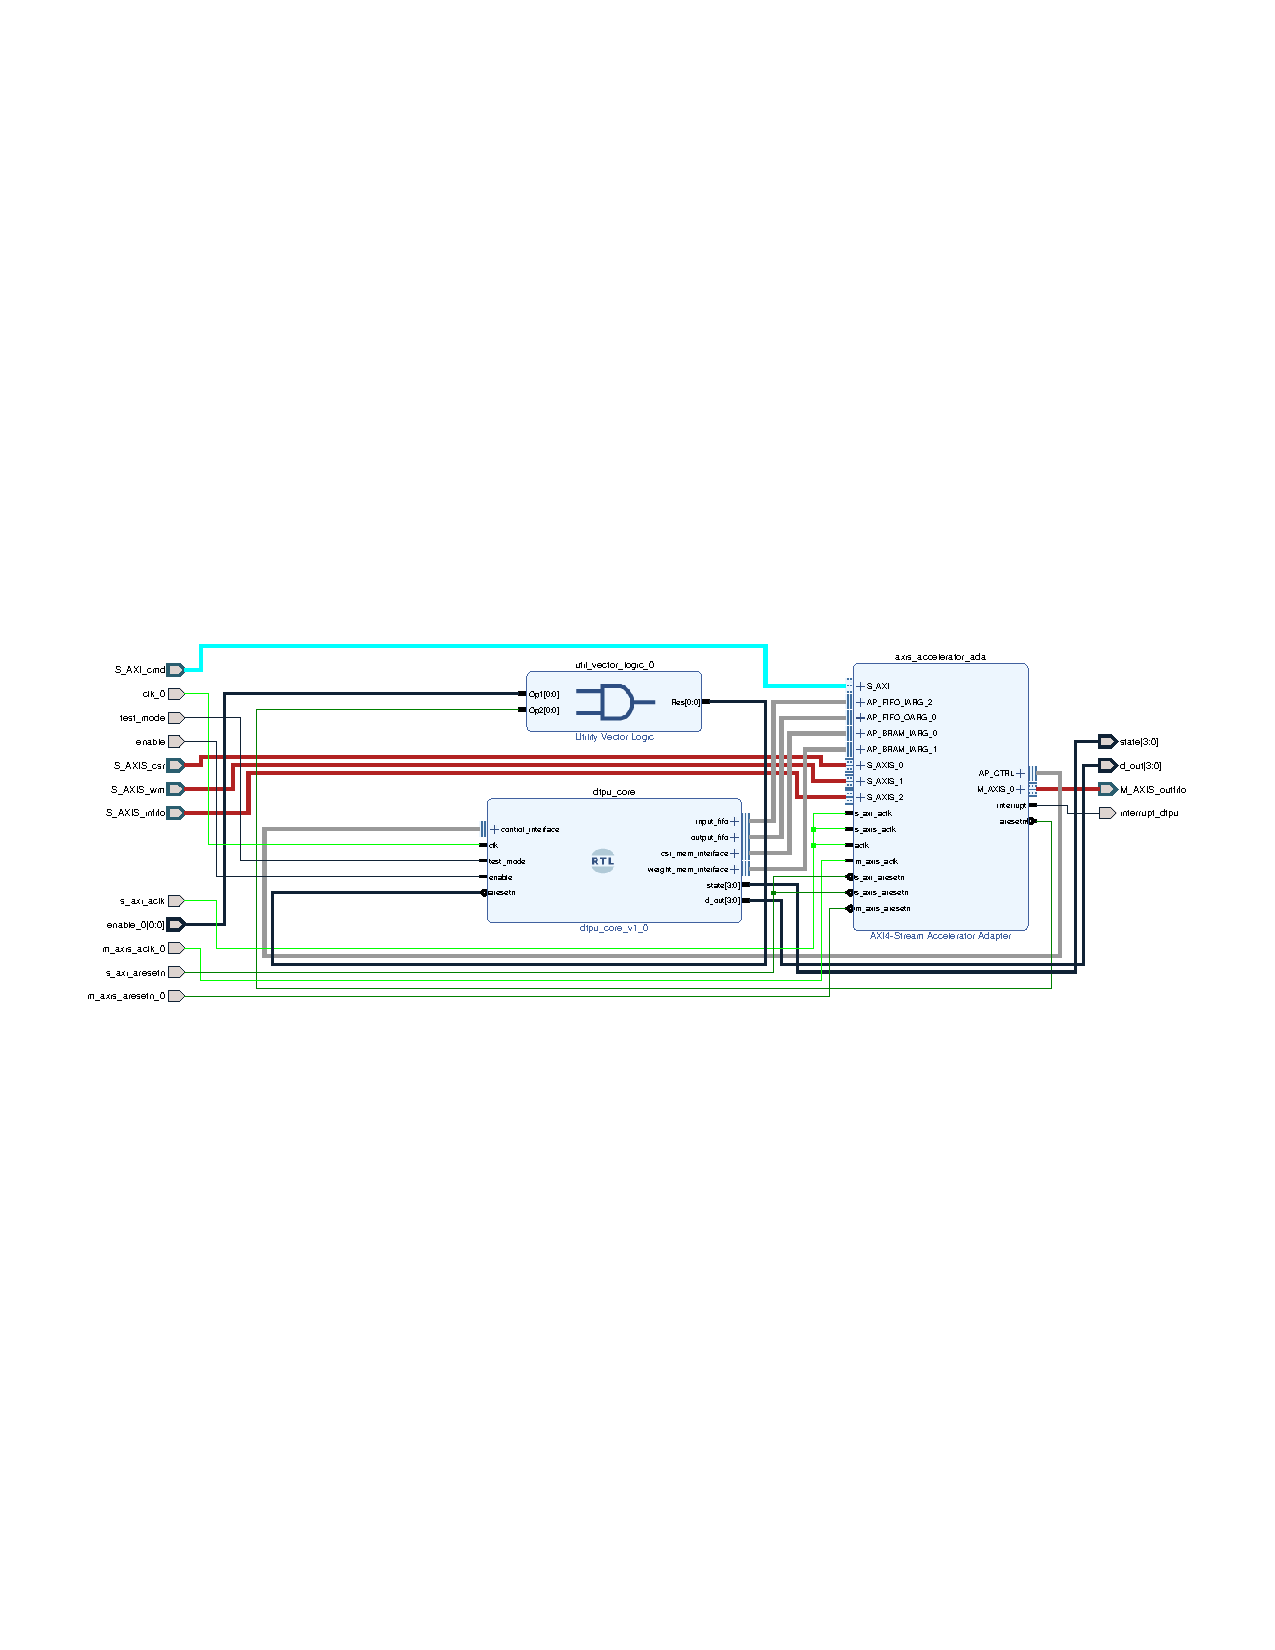
\includegraphics[scale=1,angle=90]{./figure/accelerator_schematic.pdf}
\caption{Real RTL view of the accelerator}
\label{fig:rtlaccel}
\end{figure} 
The latter has allowed to completely focus the work on the DTPU core.
\newpage
\subsection{Axi accelerator adapter}
\subsection{DTPU core}

\subsubsection{Matrix Multiplication Unit}










% RESULTS
% CREATED BY DAVID FRISK, 2016
\chapter{Results}
\textit{In this chapter, area results on the FPGA of different designs are presented. Following that, on different hardware designs Neural Network TensorFlow Lite models are executed and perfomances measured. }\\\\

\epigraph{ \textit{If you can not measure something, you can not improve it.}}{--- \textup{William Thomson Kelvin}}

\section{Evaluation metrics}
Generally speaking in Computer Science, every domain and application could have different evaluation metrics, for example the energy efficient of a CPU is a heavy metrics in embedded systems while in a high performant CPU latency and throughput are dominant metrics. As said that, evaluation metrics strongly depend on the end-users, therefore the designers have to make assumption on the end-user intentions and applications.\\
In this work the assumptions are that the accelerator will be deployed into an embedded system and at the same time it should give to the user a certain degree of flexibility for running Neural Network models. Thus, as it is suggested \cite{paper:1} the following metrics are used:
\begin{itemize}
\item Accuracy, quality of the final result of inference process.
\item Throughput, for measuring real time performance. It depends on the number of internal computation cores.
\item Latency, for interactive applications.
\item Energy and Power, for a mobile device in which there is a limited battery capacity meanwhile for data centers stringent power ceilings due to cooling costs.
\item Hardware cost (Utilization Factor in case of an FPGA) of chip area and process technology.
\end{itemize}
\newpage
\section{Utilization Factor}
An important aspect of an embedded system is the on-die utilization area. Those kinds of system are usually deployed on tightly area constrained chips for hiding their presence to the user.
Therefore, it is important to measure and understand the behavior on the Utilization of the FPGA (used as area measurement in this case) of the design as the size of Matrix Multiplication Unit increases and in parallel the throughput.\\
The Utilization Factor, composed of Look-up-Table, Flip Flops and Digital Signal Processor usage, is expected to increase as the size of Multiplication Matrix increase and the bit width of Computation Unit.
\begin{center}
\begin{tabular}{ |p{3cm}||p{3cm}|p{3cm}|p{3cm}| }
\hline
\multicolumn{4}{|c|}{Post Synthesis FPGA Utilization Computation on 4 bit integer } \\
\hline
Size of Matrix Multiplication Unit& LUT &FF&DSP\\
\hline
3x3& & & \\
4x4& & & \\
5x5& & & \\
6x6& & & \\
7x7& & & \\
8x8& & & \\
10x10& & & \\
12x12& & & \\
15x15& & & \\
16x16& & & \\
20x20& & & \\
\hline
\end{tabular}
\label{table:int4ut}
\end{center}

\begin{center}
\begin{tabular}{ |p{3cm}||p{3cm}|p{3cm}|p{3cm}| }
\hline
\multicolumn{4}{|c|}{Post Synthesis FPGA Utilization Computation on 8 bit integer } \\
\hline
Size of Matrix Multiplication Unit& LUT &FF&DSP\\
\hline
3x3& & & \\
4x4& & & \\
5x5& & & \\
6x6& & & \\
7x7& & & \\
8x8& & & \\
10x10& & & \\
12x12& & & \\
15x15& & & \\
16x16& & & \\
20x20& & & \\
\hline
\end{tabular}
\label{table:int8ut}
\end{center}

%\section{Neural Networks Models}

% CONCLUSION
% CREATED BY DAVID FRISK, 2016
\chapter{Conclusion}

\section{Discussion}
A big portion of inference process for Neural Networks involves massive multiply and add computation, basic operation of tensor convolutions, and across several execution data, especially weight tensors, are reused.
As consequence, for speeding-up and reduce the power consumption (especially in mobile devices) of ML models an hardware accelerator has been developed. 
 It is also designed for accommodating different data type computation request from Neural Network models, ranging from integer8/16/32/64 to floating-point 32 and brain floating-point 16.\\\\

The approach of the work has been a hardware/software codesign in order to accomodate the high compute intensive request of Machine Learning, the tensor convolution. Therefore, the hardware core for tensor convolution has been developed from scratch, while the common components, such as memories and bus interface, have been  chosen from the avialable ones in the tools.
Moving one step at the time above in the abstraction level, the accelerator library has been developed and deployed. In order to accomplish in a fixed time, the core of the library has been developed in Python, which has been interfaced with a C-code template provided from the developers of thee ML-framework used. This has lead to an hybrid library which encapsulates a frozen Python code layer, called from the C-code, the latter is only in charge of retrieving the data and passing them to the Python layer.
Again one step above in the abstraction, the ML-framework level is reached. In this level, the most popular ML-framework, TensorFlow, has been choosen. It also offers the possibility of delegate part of the excution graph to coprossessor or GPUs. Moreover, Tensorflow pretrained models have been quantized for different bitwidth and data precision.\\\\


It is possible to build a custom hardware accelerator for a specific ML operation and then integrate it into a framework without changing the model nor the framework.
The bottom up approach and the delegate class available in Tensorflow has allowed to fully tailor a new class of hardware accelerators which can accomodate different needs (i.e. depending on which part of the model has to be accelerater). As it has been organized, changing the core software in the Python code and the core in the hardware, it can be also used for addressing different models operations. 

\section{Future Works}
For every human artifacts, there is always work to do. In addition, for Computer Engineering artifacts there is also an importart step which is the software (and in this case also of the hardware) optimization.
In particular:

\begin{itemize} 
\item Software Optimization and migration to a full C code implementation for further reducing the latency.
\item A deep software/hardware testing for finding additional bugs.
\item Power estimation using the simulation’s switching activity in order to obtain a very precise and reliable power consumption.
\item Comparison of model execution on different state-of-the-art platforms.\\
\end{itemize}

Following the previous reccomandation, the work may arrive to a competitive level such as the one of the GPUs or other hardware platforms.

% REFERENCES / BIBLIOGRAPHY
\cleardoublepage
\addcontentsline{toc}{chapter}{Bibliography}
% CREATED BY DAVID FRISK, 2016
\begin{thebibliography}{69}

\bibitem{Reference:ref1} Frisk, D. (2016) A Chalmers University of Technology Master's thesis template for \LaTeX . Unpublished.


\bibitem{article1} Deep Learning with Limited Numerical Precision, "Suyog Gupta, Ankur Agrawal, Kailash Gopalakrishnan, Pritish Narayanan"
\bibitem{article2} Mixed-precision training of deep neural networks using computational memory , Nandakumar S. R., Manuel Le Gallo, Irem Boybat,Bipin Rajendran, Abu Sebastian,Evangelos Eleftheriou1
\bibitem{article3} Mixed-precision architecture based on computational memory for training deep neural networks, S. R. Nandakumar, Manuel Le Gallo, Irem Boybat, Bipin Rajendran†, Abu Sebastian and Evangelos Eleftherin
\bibitem{article3} Scaling Neural Machine Translation, Myle Ott, Sergey Edunov, David Grangier, Michael Auli
* INTRODUCTION TO MIXED PRECISION TRAINING, Dusan Stosic, NVIDIA
\bibitem{article4} MIXED PRECISION TRAINING, Sharan Narang, Gregory Diamos, Erich Elseny, Paulius Micikevicius, Jonah Alben, David Garcia, Boris Ginsburg, Michael Houston,Oleksii Kuchaiev, Ganesh Venkatesh, Hao Wu

\bibitem{article5}  Deep Learning Inference Using Intel® FPGAs,  Philip Colangelo, Nasibeh Nasiri, Asit Mishra, Eriko Nurvitadhi, Martin Margala, Kevin Nealis
\bibitem{article6} Efficient Fixed/Floating-Point Merged Mixed-Precision Multiply-Accumulate Unit for Deep Learning Processors, Hao Zhang , Hyuk Jae Lee  and Seok-Bum Ko 
\bibitem{article7} Rethinking floating point for deep learning, Jeff Johnson Facebook AI Research
\bibitem{article8} DEEP COMPRESSION: COMPRESSING DEEP NEURAL NETWORKS WITH PRUNING, TRAINED QUANTIZATION AND HUFFMAN CODING , Song Han, Huizi Mao ,William J. Dally
\bibitem{article9} DEEP LEARNING PERFORMANCE , User Guide, NVIDIA


\bibitem{article10} Timeloop: A Systematic Approach to DNN Accelerator Evaluation, Angshuman Parashar, Priyanka Raina, Yakun Sophia Shao, Yu-Hsin Chen, Victor A. Ying, Anurag Mukkara, Rangharajan Venkatesan, Brucek Khailany ,Stephen W. Keckler, Joel Emer
\bibitem{article11} The Deep Learning Revolution and Its for Comput er Architecture and Chip Design, Jeffrey Dean , Google Research
\bibitem{article12} Harnessing Numerical Flexibility for Deep Learning on FPGAs, Andrew C. Ling , Mohamed S. Abdelfattah, Andrew Bitar,David Han, Roberto Dicecco, Suchit Subhaschandra, Chris N Johnson, Dmitry Denisenko, Josh Fender, Gordon R. Chiu
 \bibitem{article13} MIXED PRECISION TRAINING OF DEEP NEURAL NETWORKS ,Carl Case, NVIDIA
\bibitem{article14} MLPERF INFERENCE BENCHMARK, Vijay Janapa Reddi , Christine Cheng , David Kanter ,Peter Mattson , Guenther Schmuelling , Carole-JeanWu , Brian Anderson , Maximilien Breughe , Mark Charlebois , William Chou , Ramesh   hukka , Cody Coleman , Sam Davis , Pan Deng , Greg Diamos ,Jared Duke , Dave Fick , J. Scott Gardner , Itay Hubara , Sachin Idgunji , Thomas B. Jablin , Jeff Jiao , Tom St. John , Pankaj Kanwar , David Lee ,  effery Liao , Anton Lokhmotov ,Francisco Massa , Peng Meng , Paulius Micikevicius , Colin Osborne , Gennady Pekhimenko , Arun Tejusve Raghunath Rajan ,Dilip Sequeira , Ashish Sirasao , Fei Sun ,Hanlin Tang  ,Michael Thomson , Frank Wei , EphremWu , Lingjie Xu , Koichi Yamada , Bing Yu ,George Yuan , Aaron Zhong , Peizhao Zhang , Yuchen Zhou 
\bibitem{article15} Stream Semantic Registers: A Lightweight RISC-V ISA Extension Achieving Full Compute Utilization in Single-Issue Cores , Fabian Schuiki, Florian Zaruba, Torsten Hoefler, and Luca Benini
\bibitem{article16} A Domain-Specific Architecture for Deep Neural Networks , NORMAN P. JOUPPI, CLIFF YOUNG, NISHANT PATIL, AND DAVID PATTERSON
\bibitem{article17} MIXED PRECISION TRAINING OF CONVOLUTIONAL NEURAL NETWORKS USING INTEGER OPERATIONS, Dipankar Das, Naveen Mellempudi, Dheevatsa Mudigere, Dhiraj Kalamkar, Sasikanth Avancha, Kunal Banerjee, Srinivas Sridharan, Karthik Vaidyanathan, Bharat Kaul, Evangelos Georganas, Alexander Heinecke, Pradeep Dubey, Nikita Shustrov, Roma Dubtsov, Evarist Fomenko, Vadim Pirogov, Jesus Corbal
\bibitem{article18} Fine-Grained Exploitation of Mixed Precision for Faster CNN Training
\bibitem{article19} Yongming Shen, Michael Ferdman, and Peter Milder. Maximizing CNN  accelerator  efficiency through resource partitioning.
\bibitem{article20} Yufei Ma, Yu Cao, Sarma Vrudhula, and Jae-sun Seo. Optimizing loop operation and ataflow in FPGA acceleration of deep convolutional neural networks.
\bibitem{article21} Mohammad Motamedi, Philipp Gysel, Venkatesh Akella, and Soheil Ghiasi. Design space exploration of FPGA-based deep convolutional  neural networks.  
\bibitem{article22} Hyoukjun Kwon, Ananda Samajdar, and Tushar Krishna. Maeri: Enabling flexible dataflow mapping over dnn accelerators via reconfigurable interconnects.
\bibitem{article23} Dally, W. High-performance hardware for machine learning. Invited talk at Cadence ENN Summit (Santa Clara, CA, Feb. 9, 2016)
\bibitem{article24} Han, S., Pool, J., Tran, J., and Dally, W. Learning both weights  and connections for efficient neural networks. In Proceedings of Advances in Neural Information Processing Systems (Montreal Canada, Dec.) MIT Press, Cambridge, MA, 2015
\bibitem{article25} Chen, Y., Chen, T., Xu, Z., Sun, N., and Teman, O. DianNao Family: Energy-efficient hardware accelerators for machine learning. Commun. ACM 59, 11 (Nov. 2016), 105–112. 8. Chen, Y.H., Emer, J., and Sze, V. Eyeriss: A spatial architecture for energy-efficient dataflow for  convolutional neural networks. In Proceedings of the 43rd ACM/IEEE International Symposium on Computer Architecture (Seoul, Korea), IEEE Press, 2016.
\bibitem{article26} Ienne, P., Cornu, T., and Kuhn, G. Special-purpose digital hardware for neural networks: An architectural survey. Journal of VLSI Signal Processing Systems for Signal, Image and Video Technology 13, 1 (1996), 5–25.
\bibitem{article27} Atul Rahman, Sangyun Oh, Jongeun Lee, and Kiyoung Choi. Design space exploration of FPGA accelerators for convolutional neural networks.  





\end{thebibliography}


% APPENDICES
\cleardoublepage
\appendix
\setcounter{page}{1}
\pagenumbering{Roman}			% Capitalized roman numbering starting from I (one)

% CREATED BY DAVID FRISK, 2016
\chapter{Accelerator library}

\definecolor{commentsColor}{rgb}{0.497495, 0.497587, 0.497464}
\definecolor{keywordsColor}{rgb}{0.000000, 0.000000, 0.635294}
\definecolor{stringColor}{rgb}{0.558215, 0.000000, 0.135316}


\definecolor{vgreen}{RGB}{104,180,104}
\definecolor{vblue}{RGB}{49,49,255}
\definecolor{vorange}{RGB}{255,143,102}

Script for creating library:
\lstinputlisting[  backgroundcolor=\color{white},   % choose the background color; you must add \usepackage{color} or \usepackage{xcolor}
  basicstyle=\footnotesize,        % the size of the fonts that are used for the code
  breakatwhitespace=false,         % sets if automatic breaks should only happen at whitespace
  breaklines=true,                 % sets automatic line breaking
  captionpos=b,                    % sets the caption-position to bottom
  commentstyle=\color{commentsColor}\textit,    % comment style
  deletekeywords={...},            % if you want to delete keywords from the given language
  escapeinside={\%*}{*)},          % if you want to add LaTeX within your code
  extendedchars=true,              % lets you use non-ASCII characters; for 8-bits encodings only, does not work with UTF-8
%  frame=tb,	                   	   % adds a frame around the code
  keepspaces=true,                 % keeps spaces in text, useful for keeping indentation of code (possibly needs columns=flexible)
  keywordstyle=\color{keywordsColor}\bfseries,       % keyword style
  language=Python,                 % the language of the code (can be overrided per snippet)
  otherkeywords={*,...},           % if you want to add more keywords to the set
  numbers=left,                    % where to put the line-numbers; possible values are (none, left, right)
  numbersep=5pt,                   % how far the line-numbers are from the code
  numberstyle=\tiny\color{commentsColor}, % the style that is used for the line-numbers
  rulecolor=\color{black},         % if not set, the frame-color may be changed on line-breaks within not-black text (e.g. comments (green here))
  showspaces=false,                % show spaces everywhere adding particular underscores; it overrides 'showstringspaces'
  showstringspaces=false,          % underline spaces within strings only
  showtabs=false,                  % show tabs within strings adding particular underscores
  stepnumber=1,                    % the step between two line-numbers. If it's 1, each line will be numbered
  stringstyle=\color{stringColor}, % string literal style
  tabsize=2,	                   % sets default tabsize to 2 spaces
%  title=\lstname,                  % show the filename of files included with \lstinputlisting; also try caption instead of title
  columns=fixed                    % Using fixed column width (for e.g. nice alignment)
firstline=1, lastline=59]{../../dtpu/software/create_library.py}
\newpage
C++ code of the library:
\lstinputlisting[language=C++]{../../dtpu/software/DTPU_delegate.cpp}
\newpage
Frozen python code in the accelerator library:
\lstinputlisting[language=Python]{../../dtpu/software/DTPU_delegate.py}

\chapter{Top level entity of DTPU core}

\lstinputlisting[style={verilog-style}]{../../dtpu/files/dtpu_core.v}

\chapter{Results for different frequencies}

\begin{figure}[!htbp]
\centering
\captionsetup{justification=centering}
\includegraphics[scale=0.7,angle=0]{./figure/graphs/power_pldyn_div_int8_freq_50mhz.pdf}
\caption{Post Implementation Dynamic Power Consumption per entities in Programmable Logic with a clock frequency of 50 MHz and integer 8 PEs}
\label{fig:dynpowint8ent50}
\end{figure}
\begin{figure}[!htbp]
\centering
\captionsetup{justification=centering}
\includegraphics[scale=0.7,angle=0]{./figure/graphs/power_pldyn_div_int8_freq_80mhz.pdf}
\caption{Post Implementation Dynamic Power Consumption per entities in Programmable Logic with a clock frequency of 80 MHz and integer 8 PEs}
\label{fig:dynpowint8ent80}
\end{figure}
\begin{figure}[!htbp]
\centering
\captionsetup{justification=centering}
\includegraphics[scale=0.7,angle=0]{./figure/graphs/power_pldyn_div_int8_freq_100mhz.pdf}
\caption{Post Implementation Dynamic Power Consumption per entities in Programmable Logic with a clock frequency of 100 MHz and integer 8 PEs}
\label{fig:dynpowint8ent100}
\end{figure}
\begin{figure}[!htbp]
\centering
\captionsetup{justification=centering}
\includegraphics[scale=0.7,angle=0]{./figure/graphs/power_pldyn_div_int8_freq_120mhz.pdf}
\caption{Post Implementation Dynamic Power Consumption per entities in Programmable Logic with a clock frequency of 120 MHz and integer 8 PEs}
\label{fig:dynpowint8ent120}
\end{figure}

\begin{figure}[!htbp]
\centering
\captionsetup{justification=centering}
\includegraphics[scale=0.6,angle=0]{./figure/graphs/power_pldyn_div_int16_freq_50mhz.pdf}
\caption{Post Implementation Dynamic Power Consumption per entities in Programmable Logic with a clock frequency of 50 MHz and integer 16 PEs}
\label{fig:dynpowint16ent50}
\end{figure}
\begin{figure}[!htbp]
\centering
\captionsetup{justification=centering}
\includegraphics[scale=0.6,angle=0]{./figure/graphs/power_pldyn_div_int16_freq_80mhz.pdf}
\caption{Post Implementation Dynamic Power Consumption per entities in Programmable Logic with a clock frequency of 80 MHz and integer 16 PEs}
\label{fig:dynpowint16ent80}
\end{figure}
\begin{figure}[!htbp]
\centering
\captionsetup{justification=centering}
\includegraphics[scale=0.6,angle=0]{./figure/graphs/power_pldyn_div_int16_freq_100mhz.pdf}
\caption{Post Implementation Dynamic Power Consumption per entities in Programmable Logic with a clock frequency of 100 MHz and integer 16 PEs}
\label{fig:dynpowint16ent100}
\end{figure}

\begin{figure}[!htbp]
\centering
\captionsetup{justification=centering}
\includegraphics[scale=0.6,angle=0]{./figure/graphs/power_pldyn_div_int32_freq_50mhz.pdf}
\caption{Post Implementation Dynamic Power Consumption per entities in Programmable Logic with a clock frequency of 50 MHz and integer 32 PEs}
\label{fig:dynpowint32ent50}
\end{figure}
\begin{figure}[!htbp]
\centering
\captionsetup{justification=centering}
\includegraphics[scale=0.6,angle=0]{./figure/graphs/power_pldyn_div_int32_freq_80mhz.pdf}
\caption{Post Implementation Dynamic Power Consumption per entities in Programmable Logic with a clock frequency of 80 MHz and integer 32 PEs}
\label{fig:dynpowint32ent80}
\end{figure}
\begin{figure}[!htbp]
\centering
\captionsetup{justification=centering}
\includegraphics[scale=0.6,angle=0]{./figure/graphs/power_pldyn_div_int32_freq_100mhz.pdf}
\caption{Post Implementation Dynamic Power Consumption per entities in Programmable Logic with a clock frequency of 100 MHz and integer 32 PEs}
\label{fig:dynpowint32ent100}
\end{figure}

\begin{figure}[!htbp]
\centering
\captionsetup{justification=centering}
\includegraphics[scale=0.6,angle=0]{./figure/graphs/power_pldyn_div_int64_freq_50mhz.pdf}
\caption{Post Implementation Dynamic Power Consumption per entities in Programmable Logic with a clock frequency of 50 MHz and integer 64 PEs}
\label{fig:dynpowint64ent50}
\end{figure}
\begin{figure}[!htbp]
\centering
\captionsetup{justification=centering}
\includegraphics[scale=0.6,angle=0]{./figure/graphs/power_pldyn_div_int64_freq_60mhz.pdf}
\caption{Post Implementation Dynamic Power Consumption per entities in Programmable Logic with a clock frequency of 60 MHz and integer 64 PEs}
\label{fig:dynpowint64ent60}
\end{figure}




\end{document}